\documentclass{beamer}

\title{Local Multidimensional Scaling}
\subtitle{
\\ \vspace{1cm} Ashutosh Tiwari - CS18BTECH11049 \\ Polamraju Aakarsh - ES18BTECH11027
		}

%\usetheme{lucid}
\begin{document}
	\frame {
		\titlepage
		}
	
%page 2
\frame {
	\frametitle{Introduction :-}
Local multidimensional scaling(LMDS) is a method of non-linear dimensional reduction. \\ \vspace{0.4cm} In non-linear dimensional reduction we try to contruct a set of points in three-dimensional or two-dimensional space, (which can be visualized) which best represents corresponding set of points(data set) in higher dimensional space.\\  We are said to "project" the higher dimensional data-set onto three-dimensional or two-dimensional space.
	}
	
%page 3
\frame {
	\frametitle{Introduction :-}
In a visualization task, every nonlinear projection method needs to make a compromise between trustworthiness and continuity. In a trustworthy projection the visualized proximities hold in the original data as well, whereas a continuous projection visualizes all proximities of the original data. 
	}
	
%page 4
\frame {
	\frametitle{Non-Linear Dimensional Reduction :-}
In non-linear dimensionality reduction given a set of points, we assume that there exists a corresponting set of points in three-dimensional or two-dimensisonal space such that the proximities between the points are conserved. \\ \vspace{0.4cm}In essence we assume that the data of interest lie on an embedded non-linear manifold(three-dimensional or two-dimensional) within the higher-dimensional space. 
	}
	
%page 5
\frame {
	\frametitle{Multidimensional Scaling :-}
 Consider a set of N points in higher dimension, which is to be projectred in lower dimention. Let the distance between the i'th and j'th point in higher dimension space be D_{ij}. \\Our goal is to construct a set of points x$_{k}$ (k  ranges from 1 to N)  such that distance between all  x$_{i}$ and x$_{j}$ is as close to D$_{ij}$ as possible.\\ \par In order to do this we minimize the stress function, given by\\
\vspace{0.5cm} \hspace{0.9cm} S(x$_{1}$, x$_{2}$, .... , x$_{N}$) = \sum (D$_{ij}$ - \mid \mid x$_{i}$ - x$_{j}$ \mid \mid)^{2} \\ \vspace{0.5cm} What we have done till here is \textbf{Classical} Multidimentional Scaling.
 }
	
%page 6
\frame {
	\frametitle{Local Multidimensional Scaling :-}
In Local Multidimensional Scaling we modify the stress function such that we give more importance to the pairwise distances of neighbouring points, i.e. points which are closer to each other in higher dimensional space.\\ \vspace{0.3cm} Let the set of neighbouring pairs of points be $\chi$. Low weightage, w is assigned to all the pairs of point not belonging to $\chi$. Also for all such pairs D$_{ij}$ is replaced by D. \\Here w is takent o be very small and D is taken to be very large. \\In doing so we assume that points which are not neighbour are very far from each other, 
	}

%page 7
\frame {
	\frametitle{Local Multidimensional Scaling :-}
The modified stress function now looks like this:\\ \vspace{0.3cm}
S$_{L}$(x$_{1}$, x$_{2}$, .... , x$_{N}$) = \sum_{(i,j)$\in$ $\chi$} (D$_{ij}$ - \mid \mid x$_{i}$ - x$_{j}$ \mid \mid)^{2}\\ \hspace{4cm} + w\sum_{(i,j)$\notin$ $\chi$} (\mid \mid x$_{i}$ - x$_{j}$ \mid \mid - D)^{2}
\\ \vspace{0.3cm} To simplify the expression, we take w $\sim$ 1/D, and let D $\to$ $\infty$ .
Simplifing this gives:\\ \vspace{0.3cm}
S$_{L}$(x$_{1}$, x$_{2}$, .... , x$_{N}$) = \sum_{(i,j)$\in$ $\chi$} (D$_{ij}$ - \mid \mid x$_{i}$ - x$_{j}$ \mid \mid)^{2}\\ \hspace{4cm} + $\tau$ \sum_{(i,j)$\notin$ $\chi$} (\mid \mid x$_{i}$ - x$_{j}$ \mid \mid)
\\ where $\tau$ = 2wD
	}
	
%page 8
\frame {
	\frametitle{Local Multidimensional Scaling :-}
The first term in the above equation tries to preserve local structure
in the data, while the second term encourages the representations x$_{i}$, x$_{j}$ for pairs (i, j) that are non-neighbors to be farther apart. Local MDS minimizes the stress function over x$_{i}$, for fixed values of the number of neighbors and the tuning parameter $\tau$ .
	}
	
%page 9
\frame {
	\frametitle{}
	\begin{figure}
			\centering
			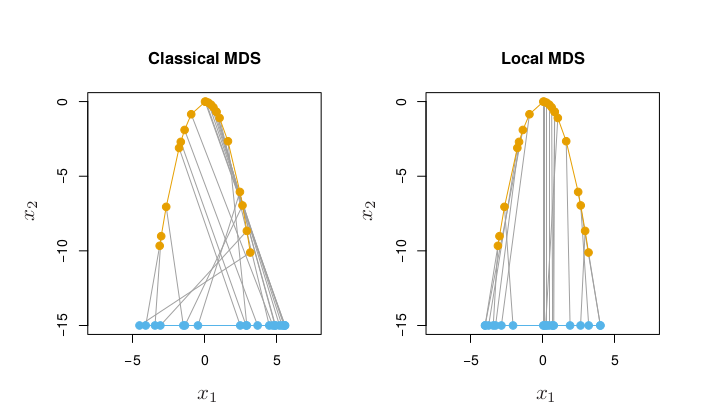
\includegraphics[scale=0.4]{image1.png}
			\end{figure}
\scriptsize{The orange points show data lying on a parabola, while the blue points shows multidimensional scaling representations in one dimension. Classical
multidimensional scaling (left panel) does not preserve the ordering of the points along the curve, because it judges points on opposite ends of the curve to be close together. In contrast, local multidimensional scaling (right panel) does a good job of preserving the ordering of the points along the curve.}
	}
	
%page 10
\frame {
	\frametitle{}
In experiments reported in Chen and Buja (2008), local MDS shows superior performance, as compared to other non dimensional reduction methods. They also demonstrate the usefulness of local MDS for graph layout. There are also close connections between the methods discussed here, spectral clustering and kernel PCA .
	}
	
%page 11
\frame {
	\frametitle{}
	\color{blue}
\hspace{3.5cm}\textsl{\Huge{Thank You!}}
	}
\end{document}